\documentclass[DIV=calc, paper=a4, fontsize=11pt, twocolumn]{scrartcl}	 % A4 paper and 11pt font size

\usepackage{multirow}
\usepackage{graphicx}
\usepackage{lipsum} % Used for inserting dummy 'Lorem ipsum' text into the template
\usepackage[english]{babel} % English language/hyphenation
\usepackage[protrusion=true,expansion=true]{microtype} % Better typography
\usepackage{amsmath,amsfonts,amsthm} % Math packages
\usepackage[svgnames]{xcolor} % Enabling colors by their 'svgnames'
\usepackage[hang, small,labelfont=bf,up,textfont=it,up]{caption} % Custom captions under/above floats in tables or figures
\usepackage{booktabs} % Horizontal rules in tables
\usepackage{fix-cm}	 % Custom font sizes - used for the initial letter in the document

\usepackage{sectsty} % Enables custom section titles
\allsectionsfont{\usefont{OT1}{phv}{b}{n}} % Change the font of all section commands

\usepackage{fancyhdr} % Needed to define custom headers/footers
\pagestyle{fancy} % Enables the custom headers/footers
\usepackage{lastpage} % Used to determine the number of pages in the document (for "Page X of Total")

% Headers - all currently empty
\lhead{}
\chead{}
\rhead{}

% Footers
\lfoot{}
\cfoot{}
\rfoot{\footnotesize Page \thepage\ of \pageref{LastPage}} % "Page 1 of 2"

\renewcommand{\headrulewidth}{0.0pt} % No header rule
\renewcommand{\footrulewidth}{0.4pt} % Thin footer rule

\usepackage{lettrine} % Package to accentuate the first letter of the text
\newcommand{\initial}[1]{ % Defines the command and style for the first letter
\lettrine[lines=3,lhang=0.3,nindent=0em]{
\color{DarkGoldenrod}
{\textsf{#1}}}{}}

%----------------------------------------------------------------------------------------
%	TITLE SECTION
%----------------------------------------------------------------------------------------

\usepackage{titling} % Allows custom title configuration

\newcommand{\HorRule}{\color{DarkGoldenrod} \rule{\linewidth}{1pt}} % Defines the gold horizontal rule around the title

\pretitle{\vspace{-30pt} \begin{flushleft} \HorRule \fontsize{50}{50} \usefont{OT1}{phv}{b}{n} \color{DarkRed} \selectfont} % Horizontal rule before the title

\title{Adder} % Your article title

\posttitle{\par\end{flushleft}\vskip 0.5em} % Whitespace under the title

\preauthor{\begin{flushleft}\large \lineskip 0.5em \usefont{OT1}{phv}{b}{sl} \color{DarkRed}} % Author font configuration

\author{Ali Alipour, } % Your name

\postauthor{\footnotesize \usefont{OT1}{phv}{m}{sl} \color{Black} % Configuration for the institution name
University of Tehran % Your institution

\par\end{flushleft}\HorRule} % Horizontal rule after the title

\date{} % Add a date here if you would like one to appear underneath the title block

%----------------------------------------------------------------------------------------

\begin{document}

\maketitle % Print the title

\thispagestyle{fancy} % Enabling the custom headers/footers for the first page 

%----------------------------------------------------------------------------------------
%	ABSTRACT
%----------------------------------------------------------------------------------------

% The first character should be within \initial{}
\initial{A}\textbf{dders play a crucial and effective role in computational tasks. The speed of computer operations greatly impacts overall performance, and optimizing these operations can significantly enhance processing speed. Therefore, various methods have been developed to reduce calculation time and accelerate processing.}

%----------------------------------------------------------------------------------------
%	ARTICLE CONTENTS
%----------------------------------------------------------------------------------------

\section*{16 bit Ladner Ficher Adder}

% \lipsum[1-3] % Dummy text

This adder belongs to the family of prefix adders and is described using VHDL. 
In Figure 1, you can see the diagram illustrating its structure.


% Insert the image in the same section
\begin{figure}[htbp]
  \centering
  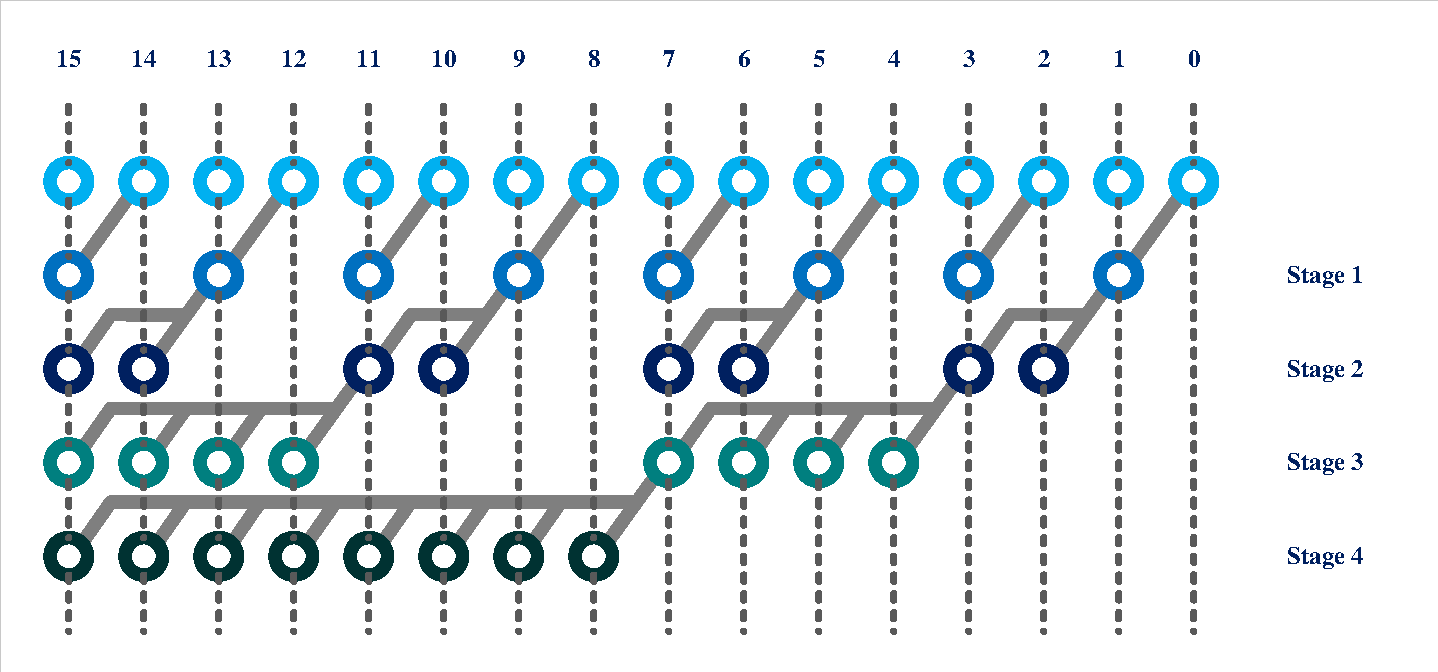
\includegraphics[width=0.4\textwidth]{C:\\Users\\USER\\Documents\\edit_project\\Adder\\Visio\\LadnerFischerAdder_16Bit.pdf}
  \caption{16 bit Ladner Ficher Adder}
  \label{fig:visio-diagram}
\end{figure}

% \begin{align}
% A = 
% \begin{bmatrix}
% A_{11} & A_{21} \\
% A_{21} & A_{22}
% \end{bmatrix}
% \end{align}

% \lipsum[4] % Dummy text

%------------------------------------------------
\section*{Binary signed with 16 digit}

% \lipsum[1-3] % Dummy text

\begin{itemize}
  \item \textcolor{red}{Note: } This method of binary decimal (BD) encoding is used in multipliers/dividers.
  \item \textcolor{red}{Note: } In BD encoded multipliers, two fewer bits are required.
\end{itemize}

% Creating the table
\[
\begin{array}{|c|c|c|c|c|}
\hline
x & x^h & x^l & x^h & x^l \\
\hline
0 & 0 & 0 & 0 & 0 \\
1 & 0 & 1 & 0 & 1 \\
\overline{1} & 1 & 0 & 1 & 1 \\
\hline
\end{array}
\]

\noindent
In this adder, we require a TW component, which operates based on the inputs from the previous stage 
(these inputs determine the value of P) and the inputs of the current stage. According to the diagram 
below, it calculates \textit{$P_{i-1},\;W_{i},\;and\;T_{i+1}$}.

\[
P_i = \left\{
    \begin{array}{ll}
        0, & \text{if } (x_i, y_i) \text{ both NonNegative } (t_{i+1} \geq 0) \\
        1, & \text{otherwise } (t_{i+1} \leq 0)
    \end{array}
\right.
\]

% Equation above the table
\[
x_i + y_i = 2 t_{i+1} + w_i
\]

% Table creation with multirow and rotated text in the first column
\begin{center}
  \begin{tabular}{|c|c|c|c|c|}
    \hline
    \multirow{6}{*}{\rotatebox{90}{\textcolor{DarkGreen}{Using Previous Digit  }}} & $x_i + y_i$ & $P_{i-1}$ & $t_{i+1}$ & $w_i$ \\
    \cline{2-5}
     & 2  & - & \multirow{2}{*}{1} & \multirow{2}{*}{1} \\
    \cline{2-3}
     & 1  & $0(t_i \geq 0)$ &  &  \\
    \cline{2-5}
     & 1  & $1(t_i \leq 0)$ & 1 & -1 \\
    \cline{2-5}
     & 0  & - & -1 & 1 \\
    \cline{2-5}
     & \multirow{2}{*}{-1} & $0(t_i \geq 0)$ & \multirow{2}{*}{-1} & \multirow{2}{*}{-1} \\
    \cline{3-3}
     &  & $1(t_i \leq 0)$ &  &  \\
    \cline{2-5}
     & -2  & - & -1 & 1 \\
    \hline
    \end{tabular}
\end{center}

% Rotated text on the side (For visual annotation, you might need to use the graphicx package)
\vspace{0.5cm}


% \[
% x = x^l \times 2^{l} + x^h
% \]

% Encoding types
% \textcolor{DarkRed}{Type 1 Encoding } \hspace{2cm} \textcolor{DarkGreen}{Type 2 Encoding }

\section*{Python Codes}

% \lipsum[8] % Dummy text

% \begin{description}
% \item[First] This is the first item
% \item[Last] This is the last item
% \end{description}

% \lipsum[9] % Dummy text

%----------------------------------------------------------------------------------------
%	REFERENCE LIST
%----------------------------------------------------------------------------------------

In Python, we implemented the Carry Lookahead Adder (CLA) in the \texttt{Carry\_Lookahead\_Adder.py} file 
and the Carry Skip Adder (CSA) in the \texttt{Carry\_Skip\_Adder.py} file. We also tested these functions 
in the \texttt{main.py} program.

\begin{thebibliography}{99} % Bibliography - this is intentionally simple in this template

  \bibitem[Alipour Fraydani and Taati, 2024]{AlipourFraydani:2024}
  Alipour Fraydani, A. and Taati, H. (2024).
  \newblock Homework on Computer Arithmetic, University of Tehran.
  \newblock {\em Unpublished Manuscript}, Department of Electrical Engineering, University of Tehran.
  
  \end{thebibliography}
%----------------------------------------------------------------------------------------

\end{document}